%% Define title of slide deck

\newcommand\CourseTopic{Introduction to R}
\newcommand\CourseTopicShort{Introduction to R}
\newcommand\CourseNumber{2}

\newcommand\CourseDate{\today}
\newcommand\CourseInstitute{ETH Zurich}
\newcommand\CourseAbbreviation{OR}
\newcommand\CourseTitle{Operations Research in R}
\newcommand\CourseAuthor{Stefan Feuerriegel}

\newcommand{\CourseQuiz}{Visit webpage with course quiz.}
\newif\ifQuizSolution\QuizSolutionfalse

\PassOptionsToPackage{table,dvipsnames}{xcolor}
\documentclass[%
  final,
  11pt, 
  show notes, % enables Notes
  t, % Place text of slides at the (vertical) top of the slides
  fleqn, % equations are centered
]{beamer} 

\usepackage{booktabs}

\newcommand\const{\mathsf{const.}}
\newcommand\rp{^{-1}}
\newcommand\rps{^{-2}}
\newcommand\rpc{^{-3}}

\newcommand\transpose{^T} %{^\top}
\newcommand\rptranspose{^{-T}} %^{^{-\top}}
\newcommand\pseudoinverse{^{+}}

\newcommand\define{:=} % :=, \ensuremath{\mathrel{\stackrel{\mathsf{def}}{=}}}
\newcommand\ldefine{=:}
\newcommand{\setsep}{\, | \,}

\newcommand{\correspond}{\mathrel{\widehat{=}}}

\newcommand{\norm}[1]{\left\Vert #1 \right\Vert}
\newcommand{\floor}[1]{\left\lfloor #1 \right\rfloor}
\newcommand{\ceil}[1]{\left\lceil #1 \right\rceil}

\newcommand{\vecval}[1]{\bm{#1}}
\newcommand{\matval}[1]{#1}

\newcommand{\sspace}{\quad}
\newcommand{\wspace}{\qquad}

\newcommand{\sand}{\sspace\text{and}\sspace}
\newcommand{\wand}{\wspace\text{and}\wspace}
\newcommand{\for}{\text{for }}

\newcommand{\R}{\mathbb{R}}
\newcommand{\N}{\mathbb{N}}

\newcommand{\unitvec}[2]{{\vecval{u}_{#1}}}
\newcommand{\identitymat}[1]{\matval{\mathup{I}}_{#1,#1}}
\newcommand{\permutemat}{\matval{\Pi}}
\newcommand{\zerovec}[1]{\vecval{0}_{#1}}
\newcommand{\zeromat}[2]{\matval{0}_{#1,#2}}

\newcommand{\fulfill}{\stackrel{!}{=}}
\newcommand{\inlineortho}{\bot}
\newcommand{\ortho}{\,\, \inlineortho \,\,}
\newcommand{\iszero}[1]{\underbrace{#1}_{=0}}

\newcommand{\vecsize}[1]{\in\R^{#1}}
\newcommand{\matsize}[2]{\in\R^{#1 \times #2}}

\newcommand{\concatmat}[1]{\Concat{#1}}
\newcommand{\concatvec}[1]{\left[#1\right]}
\newcommand{\concatmatsep}{\, | \,}
%\newcommand{\lincomb}[1]{\left\langle #1 \right\rangle}
\newcommand{\lincomb}[1]{\linearspan{#1}}
%\newcommand{\vecprod}[2]{\left( #1, #2 \right)}
\newcommand{\vecprod}[2]{\left\langle #1, #2 \right\rangle}

\newcommand{\abs}[1]{\left\lvert #1 \right\rvert}
\newcommand{\sign}[1]{\mathup{sign}\left( #1 \right)}
%\newcommand{\ssign}{\mathsf{sign}}
\newcommand{\diag}{\operatorname{diag}}
%\renewcommand\Re[1][]{\mathsf{Re}\,#1}
%\renewcommand\Im[1][]{\mathsf{Im}\,#1}

\newcommand{\vvector}[2]{\left[\begin{array}{c} #1 \\ #2 \end{array} \right]}
\newcommand{\vvvector}[3]{\left[\begin{array}{c} #1 \\ #2 \\ #3 \end{array} \right]}

\newcommand{\intervaloo}[2]{\left(#1,#2\right)}
\newcommand{\intervaloc}[2]{\left(#1,#2\right]}
\newcommand{\intervalco}[2]{\left[#1,#2\right)}
\newcommand{\intervalcc}[2]{\left[#1,#2\right]}

\newenvironment{mmatrix}{\begin{bmatrix}}{\end{bmatrix}}

\newcommand{\Oh}[1]{\mathsf{O}\left(#1\right)}

\newcommand{\e}[1]{\mathup{e}^{#1}}

\newcommand{\dd}{\mathop{}\!\mathsf{d}}
\newcommand{\Laplace}{\Updelta}

\newcommand\op[1]{{\hat{\mathsf{#1}}}}  % Operator

\newcommand\imaginary{\mathup{i}}

% use together with long limits in \sum, \prod, etc
% from mathmode, p. 63
  \def\clap#1{\hbox to 0pt{\hss#1\hss}}
  \def\mathclap{\mathpalette\mathclapinternal}
  \def\mathclapinternal#1#2{%
    \clap{$\mathsurround=0pt#1{#2}$}
  }

\newcommand\ie{i.\,e.\xspace}
\newcommand\eg{e.\,g.\xspace}
\newcommand\etc{etc.\xspace}
\newcommand\cf{cf.\xspace}

%% from: http://tex.stackexchange.com/questions/2441/how-to-add-a-forced-line-break-inside-a-table-cell
\newcommand{\mcell}[2][c]{%
  \begin{tabular}[c]{@{}#1@{}}#2\end{tabular}}
\newcommand{\mcellt}[2][c]{%
  \begin{tabular}[t]{@{}#1@{}}#2\end{tabular}}

\newcommand{\stackedcell}[2][c]{%
  \begin{tabular}[#1]{@{}c@{}}#2\end{tabular}}

<<setup, include=FALSE>>=
# change default language to display error messages in English
Sys.setenv(LANGUAGE = "en")

# smaller font size for chunks
library(knitr)
opts_chunk$set(size = "footnotesize", fig.width = 3, fig.height = 3)
@

\begin{document}

  \begin{frame}%[plain]
  \titlepage
\end{frame}
  
\begin{frame}
  \frametitle{Today's Lecture}
\vfill
\begin{block}{Objectives}
\begin{enumerate}
\item Being able to perform simple calculations in R
\item Understanding the concepts of variables
\item Handling vectors and matrices
\end{enumerate}
\end{block}
\vfill
\end{frame}
  
  % \section[Contents]{}

\begin{frame}<beamer>%[allowframebreaks]
  \frametitle{Outline}
  \tableofcontents[%
%     currentsection, % causes all sections but the current to be shown in a semi-transparent way.
%     currentsubsection, % causes all subsections but the current subsection in the current section to ...
%     hideallsubsections, % causes all subsections to be hidden.
%     hideothersubsections, % causes the subsections of sections other than the current one to be hidden.
%     part=, % part number causes the table of contents of part part number to be shown
%    pausesections, % causes a \pause command to be issued before each section. This is useful if you
%     pausesubsections, %  causes a \pause command to be issued before each subsection.
%     sections={ overlay specification },
%      sectionstyle=show/shaded,
      subsectionstyle=hide
  ]
\end{frame}

\section{General Information}

\begin{frame}
  \frametitle{Examples of Optimization Software}
\vfill
\begin{description}
  \item[Excel] Limited capabilities for optimization; good for data preprocessing
	\item[Matlab] Optimization toolbox, mainly aimed at engineering
  \item[GAMS] Optimization only, but challenging user interface
  \item[CPLEX] Optimization software package, but commercial
\end{description}
\vfill
\end{frame}

\begin{frame}
  \frametitle{What is R?}
\begin{columns}[c]
\begin{column}{.45\textwidth}
\begin{itemize}
\item Free software environment aimed at statistical computing
\item Supports many operating systems (Linux, Mac OS X, Windows)
\item Very frequently used in psychology, bioinformatics, statistics, econometrics, machine learning and optimization
\end{itemize}
\end{column}
\begin{column}{.5\textwidth}
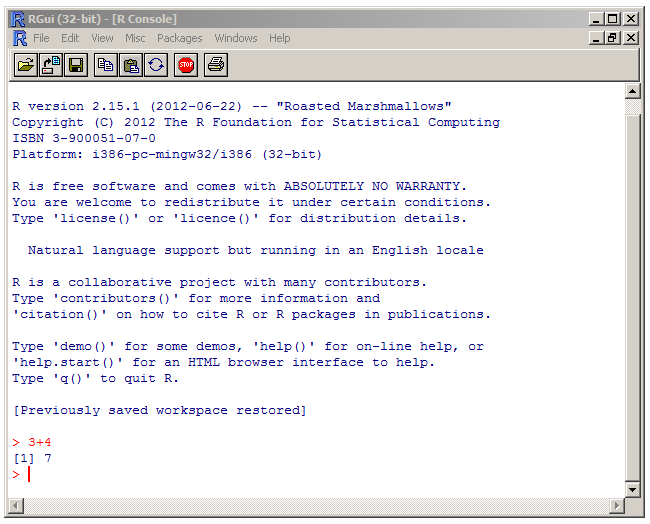
\includegraphics[width=.99\linewidth]{R-Console}
\end{column}
\end{columns}
\vfill
\begin{block}{Retrieving R}
Download at \url{http://www.r-project.org}
\end{block}
\vfill
\end{frame}

\begin{frame}
  \frametitle{R Studio as Editor}
\begin{columns}[c]
\begin{column}{.45\textwidth}
\begin{itemize}
\item Instead of typing commands into the R Console,
you can generate commands by an editor and then
\emph{send} them to the R window
\item \ldots and later modify (correct) them and send again
\end{itemize}
\end{column}
\begin{column}{.5\textwidth}
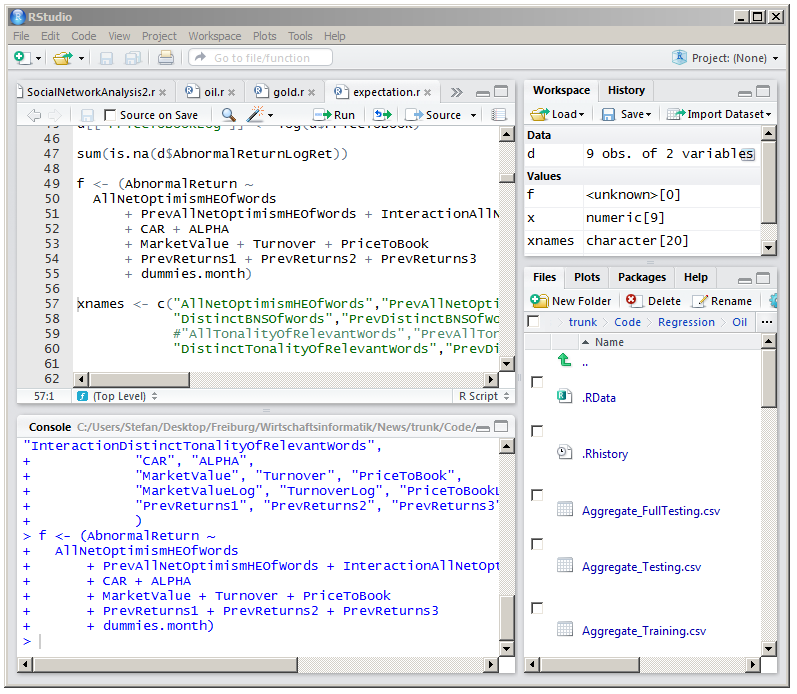
\includegraphics[width=.99\textwidth]{R-Studio}
\end{column}
\end{columns}
\vfill
\begin{block}{Retrieving R Studio (recommended)}
Download at \url{http://www.rstudio.com/}
\end{block}
\vfill
\end{frame}


\section{Operations, Functions, Variables}

\begin{frame}[fragile]
  \frametitle{First Example}
\vfill
\begin{exampleblock}{$\rightarrow$ Live Demonstration}
\end{exampleblock}
<<>>=
3*(4+2)
@
\vfill
\end{frame}

\begin{frame}[fragile]
  \frametitle{Arithmetic Operations}
\footnotesize
\begin{columns}[c]
\begin{column}{.35\textwidth}
<<,size='footnotesize'>>=
1+2*3
3/4+2
2*pi-pi
0/0
@
\end{column}
\begin{column}{.6\textwidth}
\begin{tabular}{lllr}
\toprule
\tablehead Operation &
\tablehead Description &
\tablehead Example &
\tablehead Result \tabularnewline
\midrule
\verb@+@ & Plus & \verb@3+4@ & $7$ \tabularnewline
\verb@-@ & Minus & \verb@3-4@ & $-1$ \tabularnewline
\verb@*@ & Times & \verb@3*4@ & $12$ \tabularnewline
\verb@/@ & Divide & \verb@3/4@ & $0.75$ \tabularnewline
\verb@^@ & Exponentiation & \verb@3^4@ & $3^4 = 81$ \tabularnewline
\bottomrule
\end{tabular}
\end{column}
\end{columns}
\end{frame}

\begin{frame}[fragile]
  \frametitle{Logic Operators}
\begin{block}{Comparison Operators}
Operators \lstinline{<}, \lstinline{<=}, \lstinline{==}, \lstinline{!=}, \lstinline{>=}, \lstinline{>} return boolean values \verb@TRUE@ or \verb@FALSE@
\end{block}
\begin{columns}[T]
\begin{column}{.45\textwidth}
<<>>=
3 < 4
3 > 4
3 <= 4
@
\end{column}
\begin{column}{.45\textwidth}
<<>>=
4 == 4 
3 != 4
@
\end{column}
\end{columns}
\end{frame}

\begin{frame}[fragile]
  \frametitle{Brackets, Comments and Decimal Points}
\vfill
\begin{itemize}
\item Brackets can be used to prioritize evaluations
<<>>=
3*(4+2)
@
\item Important to use a \emph{point instead of a comma}!
<<>>=
3.141
@
\item Comments via \#
<<>>=
3+4 # will be ignored
@
\end{itemize}
\vfill
\end{frame}

\begin{frame}[fragile]
  \frametitle{Mathematical Functions}
\begin{itemize}
\item Square root
<<>>=
sqrt(1+1)
@
\item Logarithm to the base $10$
<<>>=
log10(10*10*10)
@
\item Sinus function and rounding
<<>>=
sin(pi) # rarely exact: R uses limited number of digits
round(sin(pi))
@
\end{itemize}
\end{frame}

\begin{frame}[fragile]
  \frametitle{Mathematical Functions}
\vfill
\begin{center}
\begin{tabular}{lllr}
\toprule
\tablehead Function &
\tablehead Description &
\tablehead Example &
\tablehead Result \tabularnewline
\midrule
\verb@abs()@ & Absolute Value & \verb@abs(3-4)@ & $+1$ \tabularnewline
\verb@round()@ & Rounding & \verb@round(3.14)@ & $\approx 3$ \tabularnewline
\verb@sqrt()@ & Square Root & \verb@sqrt(81)@ & $\sqrt{81} = 9$ \tabularnewline
\verb@sin()@ & Sine & \verb@sin(0)@ & $\sin{0}=0$ \tabularnewline
\verb@cos()@ & Cosine & \verb@cos(0)@ & $\cos{0}=1$ \tabularnewline
\verb@tan()@ & Tangent & \verb@tan(0)@ & $\tan{0}=0$ \tabularnewline
\verb@log()@ & Natural Logarithm & \verb@log(e)@ & $\ln{\e{}} = 1$ \tabularnewline
\verb@log10()@ & Common Logarithm & \verb@log10(100)@ & $\log_{10}{100} = 2$ \tabularnewline
\bottomrule
\end{tabular}
\end{center}
\vfill
\end{frame}

\begin{frame}[fragile]
  \frametitle{Exercise: Mathematical Functions}
\vfill
\begin{exampleblock}{Question}
\begin{itemize}
\item What is the value of \verb@abs(3-4*5)@?
\item \CourseQuiz
\end{itemize}
\end{exampleblock}
\ifQuizSolution
\pause
<<>>=
abs(3-4*5)
@
\fi
\vfill
\end{frame}

\begin{frame}[fragile]
  \frametitle{Variables}
\begin{columns}[T]
\begin{column}{.35\textwidth}
<<,size='footnotesize'>>=
x <- 2
x
x+3
x
x <- x+4
x
@
\end{column}
\begin{column}{.6\textwidth}
\begin{itemize}
\item Variables store values during a session
\item Value on right is assigned to variable preceding "\verb@<-@"
\item No default output after assignment
\item Recommended names consist of letters A--Z plus "\verb@_@" and "\verb@.@"
\item Must not contain minus!
\begin{itemize}
\item Should be different from function names, \eg \verb@sin@
\item Good: \verb@x@, \verb@fit@, \verb@ratio@, \etc
\end{itemize}
\item Warning: naming is case-sensitive 
\begin{itemize}
\item \ie \verb@x@ and \verb@X@ are different
\end{itemize}
\end{itemize}
\end{column}
\end{columns}
\end{frame}

%\begin{frame}[fragile]
%  \frametitle{Exercise I: Variables}
%\vfill
%<<>>=
%x <- 2
%y <- 3
%z <- x+y
%@
%\pause
%<<>>=
%z
%x <- 10
%@
%\pause
%<<>>=
%z
%@
%\vfill
%\end{frame}

\begin{frame}[fragile]
  \frametitle{Exercise: Variables}
\vfill
\begin{exampleblock}{Question}
\begin{itemize}
\item What is the value of \verb@z@?
\item \CourseQuiz
\end{itemize}
\end{exampleblock}
<<>>=
x <- 2
x <- x+1
y <- 4
z <- x+y
x <- x+1
z <- z+x
@
\ifQuizSolution
\pause
<<>>=
z
@
\fi
\vfill
\end{frame}

\begin{frame}[fragile]
  \frametitle{Strings}
\begin{itemize}
\item Sequence of characters are named \emph{strings}
\item Surrounded by double quotes (\verb@"@)
\item Necessary for \eg naming column names
\end{itemize}
<<>>=
"Text"
"3.14"
"3.14"+1 # mixing strings and numbers does not work
@
\end{frame}

\begin{frame}[fragile]
  \frametitle{Help Pages}
Accessing help pages for each function via \verb@help(func)@
<<,eval=FALSE>>=
help(sin)
@
\begin{center}
\fbox{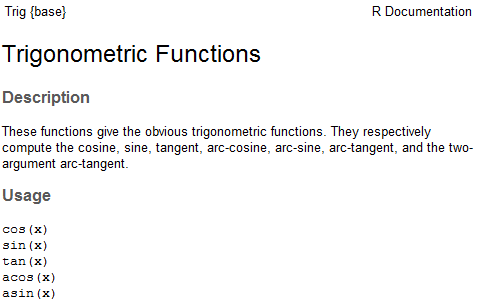
\includegraphics[width=.6\linewidth]{help_sin}}
\end{center}
\end{frame}


\section{Vectors}

\begin{frame}[fragile]
  \frametitle{Creating and Accessing Vectors}
\begin{columns}[T]
\begin{column}{.45\textwidth}\begin{itemize}
\item Create vector filled with zeros via \verb@numeric(n)@
<<>>=
numeric(4)
@
\item Vector elements are \emph{concatenated} via \verb@c(...)@
<<>>=
x <- c(4, 0, 6)
x
@
\item Accessing individual elements via squared brackets \verb@[]@
<<>>=
x[1] # first component
@
%x[3] # third component
\end{itemize}
\end{column}
\begin{column}{.45\textwidth}
\begin{itemize}
\item Selecting a \emph{range} of elements
<<>>=
x[c(2,3)]
@
\item Selecting \emph{everything but a subset} of elements
<<>>=
x[-1]
x[-c(2,3)]
@
\item Dimension via \verb@length()@
<<>>=
length(x)
@
\end{itemize}
\end{column}
\end{columns}
\end{frame}

\begin{frame}[fragile]
\frametitle{Updating Vectors}
<<>>=
x <- c(4, 0, 6)
@
\begin{itemize}
\item Replacing values
<<>>=
x[1] <- 2 # replace first component
x
@
\item Appending elements
<<>>=
y <- c(x, 8) # append an element
y
@
\end{itemize}
\end{frame}

\begin{frame}[fragile]
  \frametitle{Vectors: Concatenation}
<<>>=
x <- c(4, 0, 6)
y <- c(8, 9)
@
\begin{itemize}
\item Combining several vectors is named \emph{concatenation}
<<>>=
z <- c(x, y) # concatenating two vectors
z
@
\item Replicating elements by \verb@rep(val, count)@ to form vectors
<<>>=
rep(1, 5) # 5-fold replication of the value 1
rep(c(1, 2), 3) # repeat vector 3 times
@
\end{itemize}
\end{frame}

\begin{frame}[fragile]
  \frametitle{Vector Functions}
<<>>=
x <- c(1, 2, 3, 0, 10)
@
\begin{itemize}
\item Average value
<<>>=
mean(x)
@
\item Variance
<<>>=
var(x)
@
\item Sum of all elements
<<>>=
sum(x)
@
\end{itemize}
\end{frame}

\begin{frame}[fragile]
  \frametitle{Exercise: Vectors}
\vfill
\begin{exampleblock}{Question}
\begin{itemize}
\item How to compute a standard deviation of $x = \vvvector{1}{4}{9}$?
\begin{itemize}
\item \verb@sqr(var(x))@
\item \verb@sqrt(var(x))@
\item \verb@sd(x)@
\end{itemize}
\item \CourseQuiz
\end{itemize}
\end{exampleblock}
\ifQuizSolution
<<>>=
x <- c(1, 4, 9)
@
\pause
\begin{columns}[c]
\begin{column}{.45\textwidth}
Solution A
<<>>=
sqrt(var(x))
@
\end{column}
\begin{column}{.45\textwidth}
Solution B
<<>>=
sd(x)
@
\end{column}
\end{columns}
\fi
\vfill
\end{frame}

\begin{frame}[fragile]
  \frametitle{Vector Operations}
<<>>=
x <- c(1, 2)
y <- c(5, 6)
@
\begin{itemize}
\item Scaling
<<>>=
10*x
@
\item Addition
<<>>=
x+y
10+x
@
\item Be careful with functions such as \verb@sin()@ on vectors!
\end{itemize}
\end{frame}

\begin{frame}[fragile]
  \frametitle{Generating Sequences}
\begin{itemize}
\item Integer sequences
<<>>=
1:4
4:1
@
\item Arbitrary sequences
<<>>=
(1:10)/10
seq(4, 5, 0.1) # notation: start, end, step size
@
\end{itemize}
\end{frame}

\begin{frame}[fragile]
  \frametitle{Exercise: Vectors}
\vfill
\begin{exampleblock}{Question}
\begin{itemize}
\item How to compute $\sum\limits_{i=1}^{100}{i}$?
\begin{itemize}
\item \verb@sum(1:100)@
\item \verb@sum(1,100)@
\item \verb@sum(1-100)@
\end{itemize}
\item \CourseQuiz
\end{itemize}
\end{exampleblock}
\ifQuizSolution
\pause
<<>>=
sum(1:100)
@
\fi
\vfill
\end{frame}

\section{Matrices}

\begin{frame}[fragile]
  \frametitle{Matrices from Combining Vectors}
\vfill
\begin{itemize}
\item Generating matrices by combining vectors with \verb@cbind(...)@
<<>>=
height <- c(163, 186, 172)
shoe_size <- c(39, 44, 41)
m <- as.data.frame(cbind(height, shoe_size))
@
\ldots but exhausting!
\item \verb@as.data.frame(...)@ necessary to store data of different types (numeric, strings, etc.) 
\end{itemize}
\vfill
\end{frame}

\begin{frame}
  \frametitle{Files formatted as Comma Separated Values}
\vfill
\begin{itemize}
\item Support of naive Excel format is unsatisfactory
\item Recommended: Export as \emph{Comma Separated Values} (CSV)
\item In Excel via \emph{Save As} $\rightarrow$ file type is \emph{CSV (Comma separated)}
\item Then: right mouse click $\rightarrow$ \emph{Open with} $\rightarrow$ \emph{Text Editor} $\rightarrow$ Check if there are commas
\end{itemize}
\vspace*{0.3cm}
\begin{exampleblock}{Example File: persons.csv}
\ttfamily
name,height,shoesize,age\\
Julia,163,39,24\\
Robin,186,44,26\\
Kevin,172,41,21\\
Max,184,43,22\\
Jerry,193,45,31
\end{exampleblock}
\vfill
\end{frame}

\begin{frame}[fragile]
  \frametitle{Matrices from Text Files}
\verb@read.csv(filename, ...)@ imports \emph{data frame from text file}
\begin{itemize}
\item \verb@header=TRUE@ specifies whether columns have names
\item \verb@sep=","@ specifies column delimiter
\item \verb@as.data.frame(...)@ guarantees output as data frame
<<,echo=-1,tidy=FALSE,size='scriptsize'>>=
setwd("../Datasets/")
d <- as.data.frame(read.csv("persons.csv", 
     header=TRUE, sep=","))
d
@
\item Alternatively, \emph{choose path to file} via \verb@file.choose()@ manually
<<,eval=FALSE,tidy=FALSE,size='scriptsize'>>=
d <- as.data.frame(read.csv(file.choose(), 
     header=TRUE, sep=","))
@
\end{itemize}
%\begin{alertblock}{One must use the slash "/" instead of the "$\backslash$"!}
%\end{alertblock}
%\vfill
\end{frame}

\begin{frame}[fragile]
  \frametitle{Output: Matrices}
\begin{itemize}
\item Show first $6$ rows only (useful for large files)
<<,size='scriptsize'>>=
head(d)
@
\item Show column names 
<<,size='scriptsize'>>=
str(d)
@
\end{itemize}
\end{frame}

\begin{frame}[fragile]
  \frametitle{Accessing Matrices}
\vfill
\begin{itemize}
\item Dimension (\#rows, \#columns) or number of rows/columns
\begin{columns}[T]
\begin{column}{.45\textwidth}
<<>>=
dim(d)
@
\end{column}
\begin{column}{.45\textwidth}
<<>>=
nrow(d)
ncol(d)
@
\end{column}
\end{columns}
\item Access columns by name
<<>>=
d$height
d[["height"]]
@
\item Accessing an individual element (notation: \#row, \#column)
<<>>=
d[1,2]
@
\end{itemize}
\vfill
\end{frame}

\begin{frame}[fragile]
  \frametitle{Selecting Elements}
\begin{itemize}
\item Using single condition to select a subset of rows
<<>>=
d[d$age > 25, ]
d[d$age == 32, ]
@
\item Connecting several conditions (\verb@&@ is and, \verb@|@ is or)
<<>>=
d[d$age < 25 & d$height <= 163, ]
@
\end{itemize}
\end{frame}


\begin{frame}[fragile]
  \frametitle{Exercise: Selecting Elements}
\vfill
\begin{exampleblock}{Question}
\begin{itemize}
\item How to select all elements with \verb@age@ $26$ or \verb@shoesize@ $45$?
\begin{itemize}
\item \verb@d[d$age = 26 | d$shoesize = 45, ]@
\item \verb@d[d$age == 26 | d$shoesize == 45, ]@
\item \verb@d[d$age == 26 | d$shoesize == 45]@
\item \verb@d[d$age == 26 & d$shoesize == 45, ]@
\end{itemize}
\item \CourseQuiz
\end{itemize}
\end{exampleblock}
\ifQuizSolution
\pause
<<>>=
d[d$age == 26 | d$shoesize == 45, ]
@
\fi
\vfill
\end{frame}

\begin{frame}[fragile]
  \frametitle{Adding Columns and Column Names}
\begin{itemize}
\item Adding columns
<<>>=
d[["heightInInch"]] <- d$height/2.51
d$heightInInch
@
\item Getting column names via \verb@colnames()@
<<>>=
colnames(d)
@
\item Updating column names
<<,tidy=FALSE>>=
colnames(d) <- c("name", "waist", "weight", "shoes", 
                 "books")
colnames(d)
@
\end{itemize}
\end{frame}


\section{Extensibility}

\begin{frame}[fragile]
  \frametitle{Extending R: Packages}
\vfill
\begin{itemize}
	\item Most routines (from \eg time series, statistical tests, plotting) are in so-called \emph{packages}
	\item Packages must be downloaded \& installed before usage
	\item When accessing routines, must be loaded via \verb@library(package)@
	\item Installing packages by clicking:
\end{itemize}
\begin{columns}[T]
\begin{column}{.45\textwidth}
\begin{block}{In R Console}
\begin{itemize}
\item Menu \emph{Packages} 
\item \emph{Install package(s) \ldots} 
\item Choose arbitrary server 
\item Choose package
\end{itemize}
\end{block}
\end{column}
\begin{column}{.45\textwidth}
\begin{block}{In R Studio}
\begin{itemize}
\item Menu \emph{Tools} 
\item \emph{Install packages} 
\item Enter package name in middle input box 
\item Press \emph{Install}
\end{itemize}
\end{block}
\end{column}
\end{columns}
\end{frame}

\begin{frame}[fragile]
  \frametitle{Exercise}
\vfill
\begin{exampleblock}{Question}
\begin{itemize}
\item You are doing an analysis in R and need to use the \verb@summary()@ function but you are not exactly sure how it works. Which of the following commands should you run?
\begin{itemize}
\item \verb@help(summary)@
\item \verb@?summary@
\item \verb@man(summary)@
\item \verb@?summary()@
\end{itemize}
\item \CourseQuiz
\end{itemize}
\end{exampleblock}
\ifQuizSolution
Any of the above commands work except for \verb@man(summary)@. Make sure you always read the documentation so you know what functions do when you use them!
\fi
\vfill
\end{frame}

\section{Wrap-Up}

\begin{frame}
  \frametitle{Tutorials on Using R}
\begin{itemize}
\item Search \emph{Internet} $\rightarrow$ many tutorials available online
\item \emph{R Manual} is the official introductory document\\
{\small$\rightarrow$ \url{http://cran.r-project.org/doc/manuals/R-intro.pdf}}
\item Helpful examples and demonstrations\\
{\small $\rightarrow$ \url{http://www.statmethods.net}}
\item \emph{Help pages in R} describe parameters in detail, contain examples, but aim at advanced audience
\end{itemize}
\end{frame}

\begin{frame}
  \frametitle{Recommended Books}
\begin{itemize}
\item R in Action: Data Analysis and Graphics with R\\
(Manning, 2011, by Kabacoff, same as \url{statmethods.net})
\item R Cookbook\\
(O'Reilly, 2011, by Teetor)
\end{itemize}
\begin{center}
\begin{tabular}{ccc}

\includegraphics[width=0.35\textheight]{R_in_Action} &
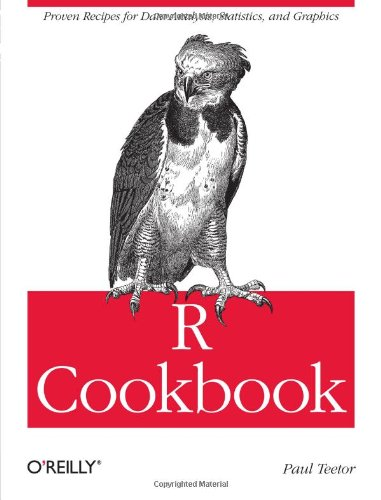
\includegraphics[width=0.35\textheight]{R_Cookbook}
\end{tabular}
\end{center}
\end{frame}

\begin{frame}[fragile]
  \frametitle{Summary: Commands}
\vfill
\begin{block}{}
\begin{tabular}{ll}
\verb@+@, \verb@-@, \etc & Algebraic operators \tabularnewline
\verb@&@, \verb@|@, \verb@<@, \verb@<=@, \etc & Logic operators \tabularnewline
\verb@help(func)@ & Help pages \tabularnewline
\verb@mean()@, \verb@var()@ & Functions on vectors \tabularnewline
\verb@sd()@ & Standard deviation \tabularnewline
\verb@seq()@ & Generate sequences \tabularnewline
\verb@d$column@ & Accessing columns of a matrix \tabularnewline
\verb@read.csv()@ & Reading text files \tabularnewline
\end{tabular}
\end{block}
\vfill
\end{frame}

%\begin{frame}
  %\frametitle{Outlook}
%\vfill
%\begin{block}{Additional Materials}
%\begin{itemize}
%\item Short summary of today's lecture $\rightarrow$ \emph{Seminar Paper}
%\item Further exercises in homework~1
%\end{itemize}
%\end{block}
%\vfill
%\begin{block}{Future Exercises}
%R will be used to solve sample optimization problems
%\end{block}
%\vfill
%\end{frame}

\end{document}

